\documentclass[11pt,a4paper]{article}
\usepackage[margin=2cm]{geometry}
\usepackage[T1]{fontenc}\usepackage[utf8]{inputenc}\usepackage{lmodern,microtype}
\usepackage{amsmath,amssymb,mathtools}
\usepackage{booktabs,tabularx,longtable,array,graphicx,float,enumitem,xcolor,hyperref,fancyhdr,titlesec}
\usepackage[backend=biber,style=numeric-comp,sorting=none]{biblatex}\addbibresource{references.bib}
\usepackage[most]{tcolorbox}
\definecolor{deepblue}{RGB}{28,63,105}\definecolor{deepgreen}{RGB}{38,105,79}\definecolor{deeporange}{RGB}{170,92,20}\definecolor{deepred}{RGB}{145,52,52}
\definecolor{softblue}{RGB}{232,241,250}\definecolor{softgreen}{RGB}{235,247,240}\definecolor{softorange}{RGB}{253,243,226}\definecolor{softred}{RGB}{252,235,235}
\hypersetup{colorlinks=true,linkcolor=deepblue,citecolor=deepgreen,urlcolor=deeporange,pdftitle={Geometry-MMALS G1 Reviewer Report v1.3},pdfauthor={Guillaume Harbonnier}}
\pagestyle{fancy}\fancyhf{}\lhead{Geometry-MMALS G1}\rhead{Reviewer report v1.3}\cfoot{\thepage}\setlength{\headheight}{14pt}
\titleformat{\section}{\Large\bfseries\color{deepblue}}{\thesection}{.8em}{}\titleformat{\subsection}{\large\bfseries\color{deepgreen}}{\thesubsection}{.8em}{}
\renewcommand{\arraystretch}{1.15}\newcolumntype{Y}{>{\raggedright\arraybackslash}X}
\newtcolorbox{positivebox}[1][]{title={#1},colback=softgreen,colframe=deepgreen!45,boxrule=.6pt,arc=2pt}
\newtcolorbox{warningbox}[1][]{title={#1},colback=softorange,colframe=deeporange!50,boxrule=.6pt,arc=2pt}
\newtcolorbox{criticalbox}[1][]{title={#1},colback=softred,colframe=deepred!50,boxrule=.6pt,arc=2pt}
\newtcolorbox{plainbox}[1][]{title={#1},colback=softblue,colframe=deepblue!45,boxrule=.6pt,arc=2pt}
\begin{document}
\begin{titlepage}\centering
\vspace*{1cm}{\Huge\bfseries\color{deepblue} Geometry-MMALS G1\par}\vspace{.2cm}
{\LARGE Status and Perspective Reviewer Report v1.3\par}\vspace{.35cm}
{\Large Updated through the executed v1.1.0 five-seed functional-routing pilot\par}\vspace{.8cm}
{\Large Guillaume Harbonnier\par}\vspace{.2cm}
{\normalsize Independent research status document - June 2026\par}
\vfill
\begin{minipage}{.92\textwidth}\small
\textbf{Reviewer verdict.} The program now has replicated candidate evidence for context geometry and partial evidence that low-capacity routing transmits that order into routes. The prototype-energy router passes trained-factor nominal and functional mediation gates and generalizes nominally to held-out angles, but held-out functional mediation is null. A linear router is at least as competitive and produces stronger exploratory causal and ablation signals. Causal specificity, mature host ecology, memory transport, and operational superiority remain unqualified. The correct next step is a bridge-isolation experiment, not a larger qualification run.
\end{minipage}\vfill
\end{titlepage}
\tableofcontents\clearpage

\section{Executive assessment}
\begin{positivebox}[What changed since reviewer report v1.2]
v1.2 ended with a replicated context map and a missing context-to-route bridge. v1.1.0 now shows that the bridge can be partially built: low-capacity routers preserve more factor order than the MLP while reading the exact same frozen context. This is the first replicated route-mediation result in the program.
\end{positivebox}

\begin{warningbox}[Why the claim must remain narrow]
The prototype effect is functionally positive only on trained factor values. It does not generalize under the current functional metric to held-out angles, fails causal-specificity and prediction-identity gates, and does not establish specialized host functions or operational value.
\end{warningbox}

\section{Evidence ladder}
\begin{table}[H]\centering\small
\begin{tabularx}{\textwidth}{lYY}
\toprule
Level & Question & Current status\\\midrule
Representational & Does the inferred context reflect rotation order and generalize across source identities? & Replicated candidate pass from v1.0.9.\\
Structural routing & Does route order inherit some context order? & Candidate pass in v1.1.0, strongest for low-capacity routers.\\
Functional routing & Do route changes correspond to ordered movement among distinct host functions? & Partial on trained factors; held-out result null.\\
Causal host control & Are tangent interventions specific and identity preserving? & Fail for prototype; exploratory linear signal unstable.\\
Host ecology & Do territories correspond to reproducible competencies? & Fail.\\
Operational utility & Does the chain improve accuracy, forgetting, robustness, or cost? & Not demonstrated.\\
Memory transport & Are route-function relations preserved across continual updates? & Not implemented.\\
\bottomrule
\end{tabularx}
\end{table}

\section{Protocol integrity}
The five-seed pilot uses matched compute, identical frozen context checkpoints within each seed, common initial host/classifier states, disjoint source partitions, and no angle-supervised route loss in the primary routing comparison. Every treatment uses 15,360 forward images and 80 optimizer steps per seed. Context preservation is exact to recorded numerical precision.

\section{Core quantitative results}
\subsection{Method means}
\begin{figure}[H]\centering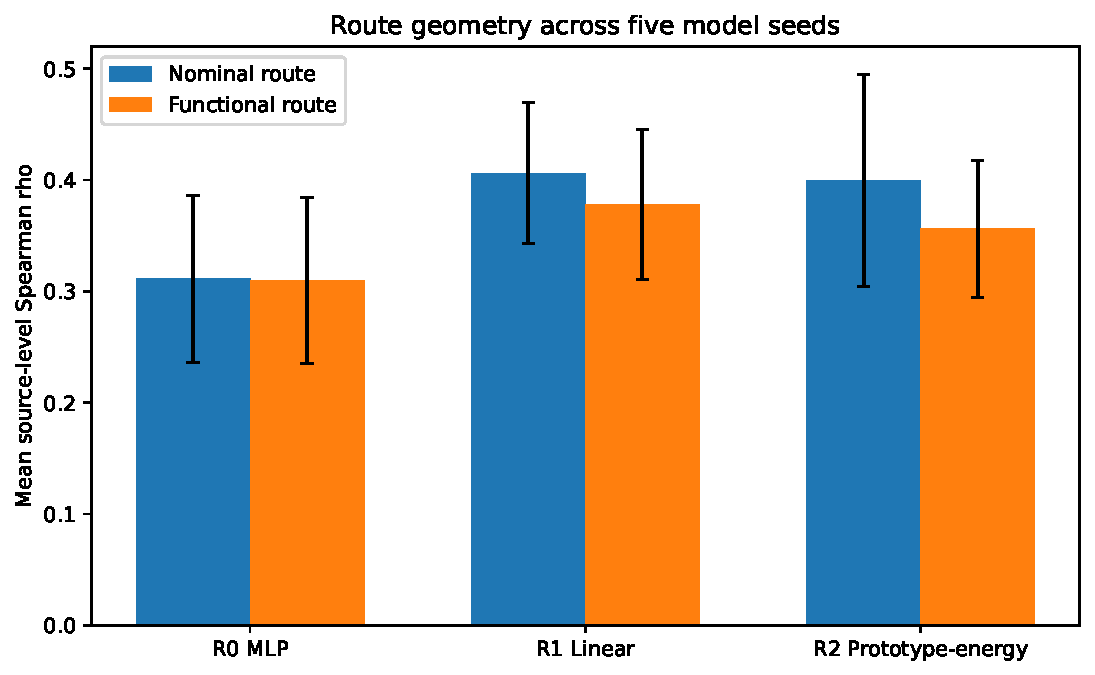
\includegraphics[width=.82\textwidth]{figures/route_geometry_summary.pdf}\caption{Five-seed route geometry summaries.}\end{figure}
\begin{table}[H]\centering\small
\begin{tabular}{lccccc}\toprule
Method & Nominal $\rho$ & Functional $\rho$ & Held-out acc. & Final acc. & Forgetting\\\midrule
MLP & 0.311 & 0.310 & 0.5692 & 0.6303 & 0.0979\\
Linear & \textbf{0.406} & \textbf{0.378} & 0.5658 & 0.6284 & 0.1012\\
Prototype-energy & 0.400 & 0.356 & 0.5668 & 0.6280 & \textbf{0.0929}\\
\bottomrule\end{tabular}
\end{table}

\subsection{Primary R2--R0 contrast}
\begin{figure}[H]\centering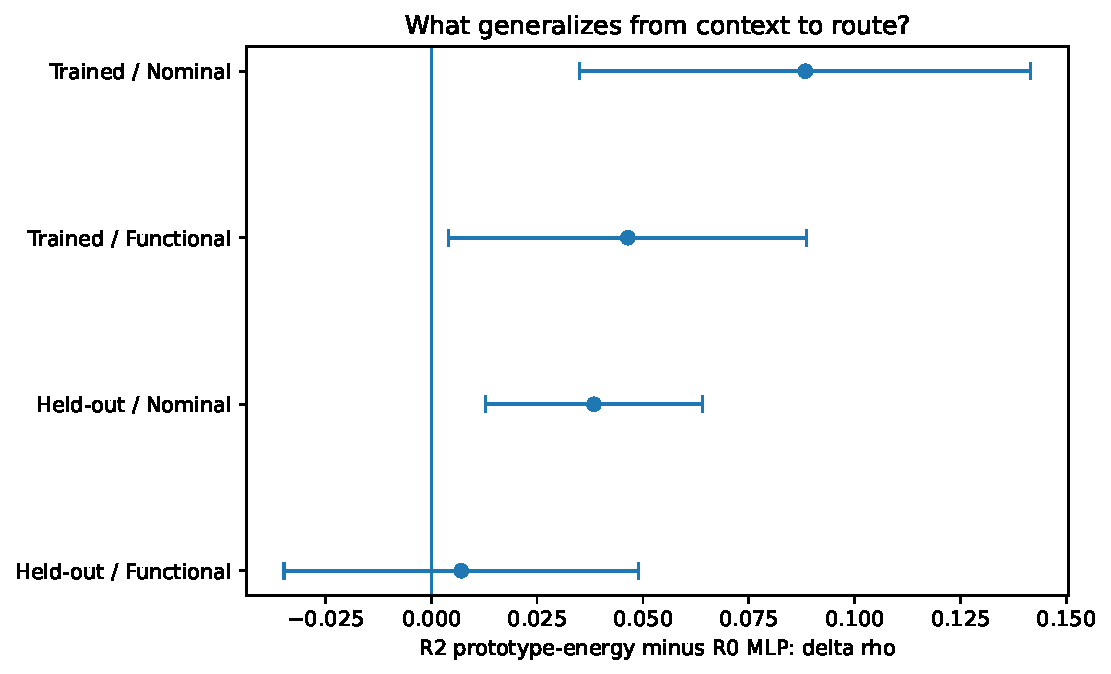
\includegraphics[width=.82\textwidth]{figures/primary_route_effects.pdf}\caption{Prototype-energy minus MLP route-order effects.}\end{figure}
The prototype improves trained nominal $\rho$ by $0.088$ ($[0.035,0.142]$), trained functional $\rho$ by $0.046$ ($[0.004,0.089]$), and held-out nominal $\rho$ by $0.038$ ($[0.013,0.064]$). The held-out functional effect is $0.007$ ($[-0.035,0.049]$).

\subsection{Linear router}
The 20-parameter linear router reaches the highest mean route correlations and a positive trained nominal effect of $0.095$ ($[0.009,0.181]$) over the MLP. It is not inferior to the 24-parameter prototype on any primary route-order mean. This is a substantive finding, not merely a baseline detail.

\section{Mechanism analysis}
\subsection{Probe controls}
\begin{figure}[H]\centering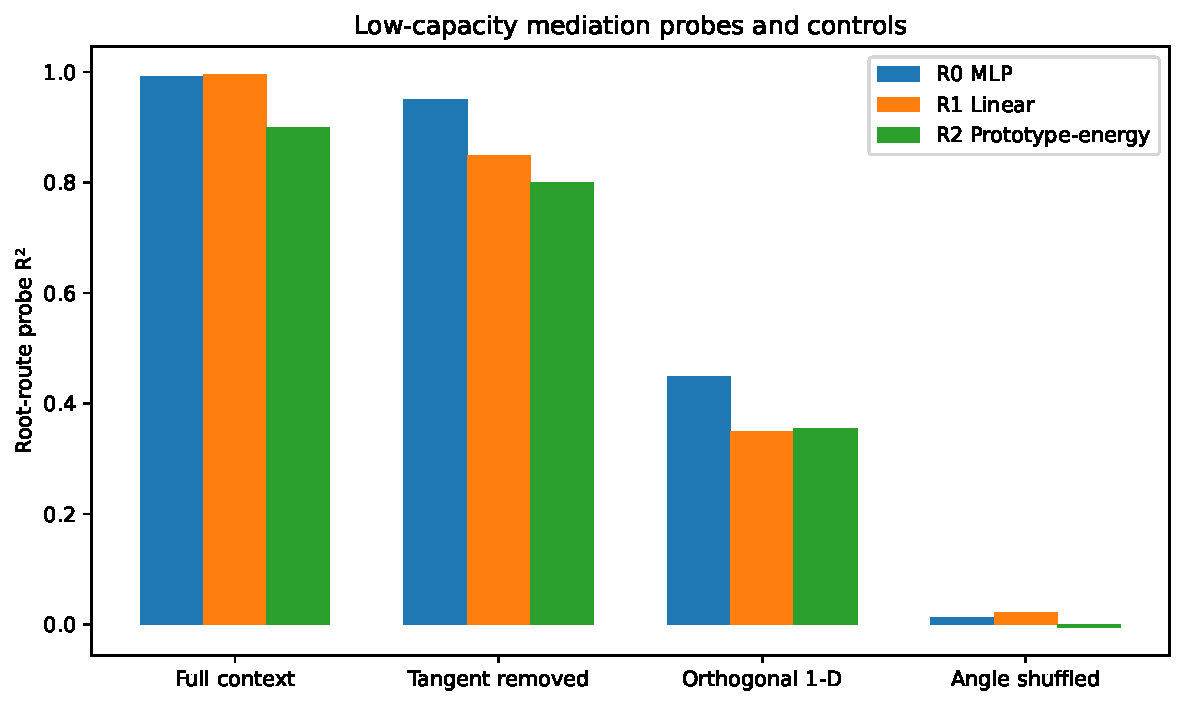
\includegraphics[width=.88\textwidth]{figures/probe_controls.pdf}\caption{Context-to-route probe controls.}\end{figure}
Full-context reconstruction is high because routes are computed from context. The scientifically useful controls are tangent removal, orthogonal projection, and factor shuffling. The linear router loses the most reconstruction after tangent removal, consistent with direct use of the factor-relevant direction.

\subsection{Causal tests}
\begin{figure}[H]\centering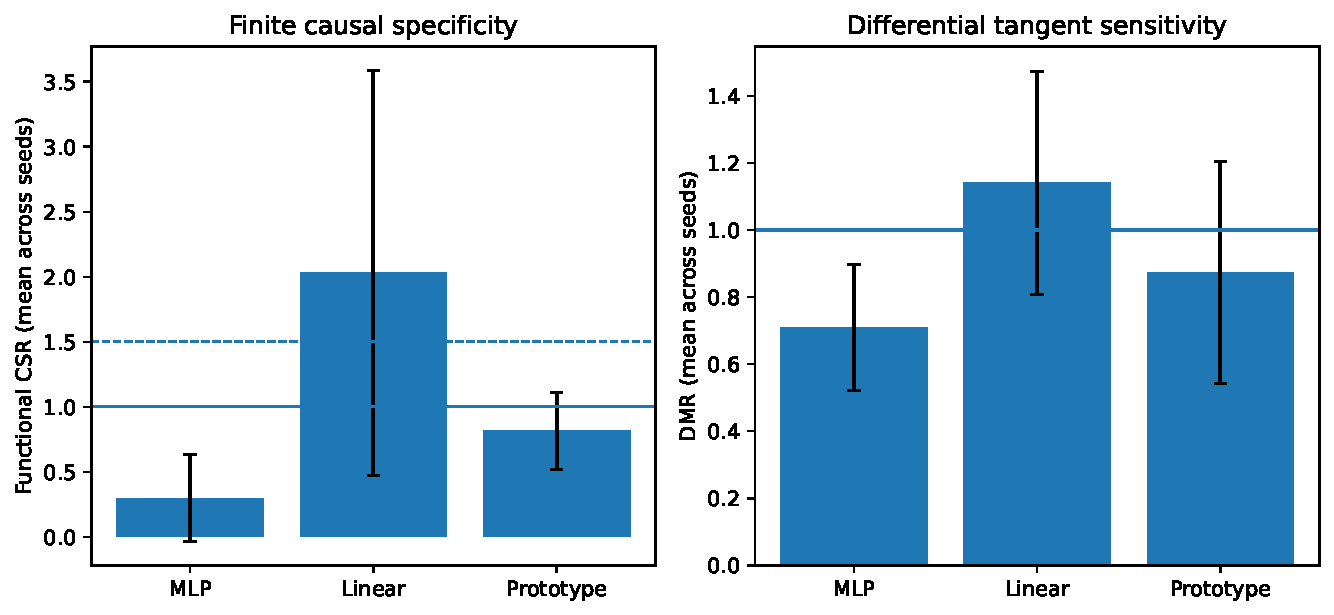
\includegraphics[width=.9\textwidth]{figures/causal_summary.pdf}\caption{Functional causal specificity and differential mediation.}\end{figure}
The prototype fails. The linear router is the strongest lead but does not pass the cross-seed source-bootstrap gate. No causal claim should be promoted.

\subsection{Host ecology}
\begin{figure}[H]\centering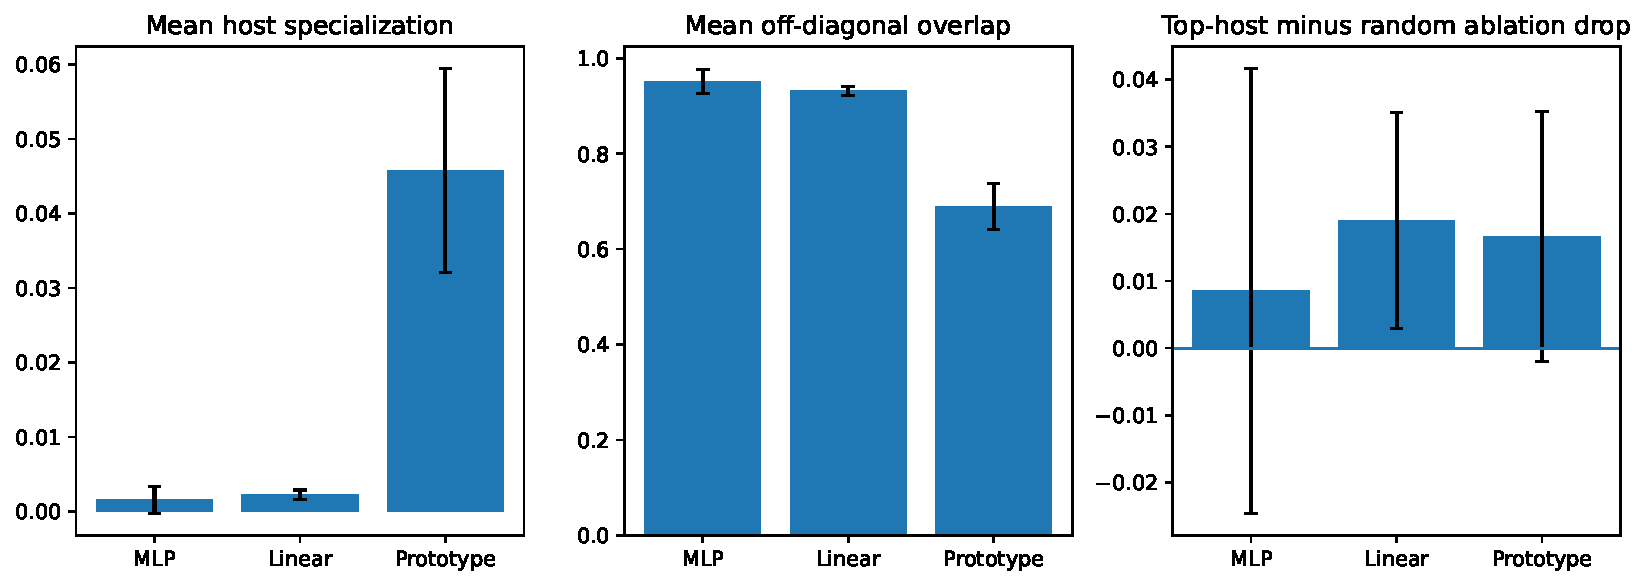
\includegraphics[width=.98\textwidth]{figures/host_ecology_summary.pdf}\caption{Territories, overlap, and ablation evidence.}\end{figure}
The prototype creates the sharpest territories but not the most reproducible functional importance. The distinction between routing specialization and functional specialization is now empirically visible.

\section{Major reviewer concerns}
\subsection{Concern 1: trained-factor functional gate}
The current functional gate can pass even though the held-out functional interval includes zero. Any generalization claim must use held-out functional mediation as primary evidence.

\subsection{Concern 2: method-specific functional cost matrices}
The functional metric is built from method-specific trained hosts. It therefore combines route movement and changing host function. The next primary comparison requires a common frozen host bank and common $C^\star$.

\subsection{Concern 3: parameter count is not the explanation}
The MLP has far more parameters, but its flexibility does not preserve geometry better. The scientifically relevant variable is inductive structure, not capacity alone. Equal-parameter controls remain useful, but the linear result already falsifies the idea that more expressive routing is automatically better.

\subsection{Concern 4: no mature host ecology}
Sharp routing territories cannot be interpreted as functional roles without contribution, ablation, swap, representation, gradient, and cross-seed role evidence.

\subsection{Concern 5: operational neutrality}
The experiment is mechanism-first and operationally neutral. That is acceptable at G1, but a publication claiming utility would require a later C6 result on at least one secondary dataset.

\section{Reviewer-safe claims}
\begin{plainbox}[Acceptable]
The routing operator exhibits measurable structure under the tested context representation and route metrics. Low-capacity linear and prototype-energy routers preserve more rotation-factor order in their route distributions than a flexible MLP, while prototype-energy routing produces a trained-factor improvement under a host-function-aware optimal-transport metric.
\end{plainbox}
\begin{criticalbox}[Not acceptable]
MMALS has learned a Riemannian manifold; prototype routing is causally superior; hosts are functionally specialized; functional mediation generalizes; geometry improves continual learning; or the energy-guided controller is qualified.
\end{criticalbox}

\section{Required v1.1.1 experiment}
The next experiment should freeze the context, host bank, classifier, and common functional cost matrix, then compare MLP, linear, prototype, and hybrid directional-prototype routers. The primary gate becomes held-out functional mediation. Additional required tests are local-continuity distributions, perturbation tails, route sensitivity maps, candidate permutation, route swaps, host deletion, tangent/orthogonal controls, and prediction identity.

The hybrid energy is
\begin{equation}
E_h(c)=\alpha\frac{d_C(c,\mu_h)^2}{2\sigma_h^2}-\beta a_h^\top c+b_h.
\end{equation}
It directly tests the interpretation suggested by v1.1.0: prototypes create local territories, while a directional term transmits the global factor coordinate.

\section{Longer plan and branch boundaries}
\begin{itemize}
\item v1.1.2: compare Euclidean, log-Euclidean, affine-invariant SPD, and simple covariance metrics for drift and specialization.
\item v1.1.3: test route-function memory, path reconstruction, and continual transport.
\item v1.1.4: qualify specialization through contribution, ablation, swaps, representation separation, and cross-seed matching.
\item G2: add host state, memory risk, cost, stability, and goals to the geometric energy.
\item TPUT: add goal-conditioned policy, future prediction, regret, and forward--backward control.
\item Verification stack: independently version metrics, check protocol validity, and assign PASS/PARTIAL/FAIL/NOT\_TESTED to every claim.
\end{itemize}

\section{Publication recommendation}
\begin{warningbox}[Recommendation]
Do not move to a broad architecture or final-paper claim yet. The evidence justifies a focused research note on replicated context geometry and partial route mediation, provided the negative held-out functional, causal, ecological, and operational results are foregrounded. For a stronger geometry-to-function paper, complete v1.1.1 first.
\end{warningbox}

\section{Updated gate table}
\begin{longtable}{p{5cm}p{2.2cm}p{7cm}}\toprule
Gate & Status & Interpretation\\\midrule\endfirsthead\toprule
Gate & Status & Interpretation\\\midrule\endhead
Context frozen and matched compute & PASS & Protocol integrity established.\\
Replicated context geometry & PARTIAL/PASS & Candidate evidence from v1.0.9, not final universal qualification.\\
Nominal route mediation & PARTIAL & Positive trained and held-out prototype effects.\\
Functional route mediation & PARTIAL & Positive on trained factors, null on held-out factors.\\
Probe controls & PARTIAL & Factor-sensitive reconstruction, not sufficient causal evidence.\\
Functional causal specificity & FAIL & Prototype below gate; linear unstable across seeds.\\
Prediction identity & FAIL for R2 & Prototype boundaries are too disruptive under intervention.\\
Host ecology & FAIL & Territories without stable competencies.\\
Operational non-degradation & PASS & Equivalence only.\\
Operational superiority & NOT\_TESTED & No supported claim.\\
Memory transport & NOT\_TESTED & Planned for v1.1.3.\\
Full energy-guided control & NOT\_TESTED & Geometry term only.\\
\bottomrule\end{longtable}

\section{Final verdict}
The program is progressing scientifically because each version narrows the uncertainty. v1.0.9 established the map. v1.1.0 established that simple routers can begin to follow it. The new bottleneck is not whether context geometry exists, but whether route movement can be made functionally general, causally specific, and ecologically meaningful. v1.1.1 is a well-posed falsification experiment for that bottleneck.

\printbibliography
\end{document}
